\documentclass[prc, 12pt]{revtex4-1}
 \usepackage{amsfonts}
 \usepackage{epsfig}    
 \usepackage{graphicx}  
 \graphicspath{ {./images/} }
 \usepackage{xcolor}
 \usepackage{subfigure}
 \usepackage{lineno}
 \linenumbers
 \begin{document}
 \topmargin=.05in
 \title{Report Update June 2023; Epistemology of Decoy Systems; Probing the Attacks on the Privacy of the Monero Blockchain}
 \author{Nathan Borggren}
 \affiliation{CompDec}
 \date{\today}

\begin{abstract}
In an effort to address adversarial attacks on the privacy of the Monero blockchain, in which an adversary utilizes leaked or privileged information to gain information about the global network, a mathematical and accompanying computational environment will be developed that is amenable to analytical, empirical, and simulated analysis.  The proposed work will quantify, measure, and analyze the structure and sensitivity Monero has with respect to the fungibility of the Monero coins, the connectivity of merchants and their customers, and how this structure can change as the microeconomics of repeated transactions is correlated and associated.  Results, code, and recommendations will be shared with the community with the goal of quantifying, qualifying and improving its privacy capabilities.
\end{abstract}

\maketitle{}

\textcolor{red}{The report update is included as additional comments marked in red for the sake of checking and maintaining context.}

\section{Introduction}

This proposal seeks financial and technical support to provide analysis in abstracto, in silico, and ultimately in situ of Monero's privacy features.  We seek to address the concerns raised about decoy systems in \cite{MiersZcash}.  The particular attacks raised in that work are the 

\begin{itemize}
   \item \textbf{Overseer Attack} - In which a merchant (receiver) uses their privileged transaction information to deduce repeat customers and build up a consumer model of their customers.  This may already be a severe problem given the fraction of transactions that involve an exchange as one of the counter-parties.  
   \item \textbf{Flashlight Attack} - A sender repeats transactions to an address or collection of addresses, providing them the means to link stealth addresses in the blockchain, and follow the taint tree forward to identify funds being aggregated (perhaps at a subpoena-able exchange).
   \item \textbf{Tainted Dust Attack} - Similar to a Flashlight Attack, but may involve a large number of candidate addresses, with an effort of identifying which address leads to a particular user-pattern.
\end{itemize}

though other related information leaks can also occur:

\begin{itemize}
  \item \textbf{Anomalous or unique wallet configurations.}   Users may inadvertently identify themselves by making unique choices for RingCT or number of outputs, use of flags, additional information etc.  In previous machine learning blockchain analysis, features involving these choices were a primary source of leaks, as evidenced by their preference by random forests, neural networks, and other classification schemes.
  \item \textbf{Anomalous or unique decoy selection.}  If a wallet or user uses non-standard decoy selection, the distributions used can often be teased apart from standard decoy selections by common statistical means.  
  \item \textbf{Broadcasting of private information}.  ShapeShift's API leaked a mass of information for a number of years.  Mining pools tend to broadcast information about coinbase transactions.
  \item \textbf{Mordinals and anomalous $tx\_extra$.}  Some users are indifferent or otherwise misaligned from the privacy use-case of Monero and seek to immortalize themselves on the blockchain.  This behavior has a network effect of reducing the effective ring size of subsequent transactions.  
\end{itemize}

All of these memory leaks share the common properties of leaking information about the ring inputs, the tx outputs, or both.  If the decoy system is working ideally and as intended then these effects should be localized and protect both senders and receivers from each other as well as third parties.  However, much work needs to be done to quantify, qualify, and improve the systems.  This proposal seeks to do so with a Three-Pronged Approach: Theoretical, Computational, and Experimental.  

The theoretical framework will build upon previous graph theoretical work which is largely concerned with asymptotic and/or stationary behavior.  The computational work proposes to use statistical machinery like pymc, to efficiently explore a vast number of scenarios in a controlled manner, allowing information to be incorporated into the models in a Bayesian sense and simulate the effect of introducing dramatic changes.  The empirical framework will take advantage of the test network and if deemed prudent, the real network to analyze the transaction graphs as they appear on actual blockchains.

An advantage of the multi-pronged approach is to incorporate other interested parties into the analysis as will be discussed in the final \textit{Proposal Request} section.

\textcolor{red}{
\subsection{Summary}
Progress has been made on each of the three fronts: Theoretical, Computational, and Experimental described at the end of each of their respective sections.  A technical document has been started and a computational package, called \textit{MoneroAna} has also been started.  These will be migrated to git in the coming weeks and shared with the working group.  I will also be migrating and reproducing the work in the computing environment provided by Rucknium and Gingeropolous. 
}

\textcolor{red}{
Progress includes:
\begin{itemize}
  \item monerod running and synced
  \item onion-monero-explorer instantiated and serving json
  \item \textit{MoneroAna} python package started 
     \begin{itemize}
     \item taint tree generation - a depth/breadth first search algorithm modified to yield the taint tree by likeliness
     \item taint tree sampling - A Monte Carlo tree search was designed to sample the tree quickly
     \end{itemize}
  \item Analysis note started
\end{itemize}}


\section{Theoretical Framework}
Previously there has been graph theoretical work into graph-based attacks that have provided some comfort into the viability of decoy systems \cite{egger2022defeating, vijayakumaran2021analysis}, but more effort needs to be made to see this established in the wild.  In particular the privacy loss from repeated transactions with another party needs to be quantified and measured.  Additional privacy features beyond decoys might be necessary.  

Topological Data Analysis (TDA) is an approach to algebraic topology that prioritizes the analysis of real world data.  \cite{rabadan2019topological, carlsson2009topology}  As graphs are the '1-skeleton' of the simplicial structures of algebraic topology a connection can be made with the graph theory of previous work.  In addition to the vertices and edges present in graph theory, TDA allows for higher order simplices to be constructed.  For example faces consisting of three vertices $(V_1, V_2, V_3)$ can aid in incorporating the additional information gained in situations like the Overseer Attack and the Eve-Alice-Bob-Eve (EABE) Attack and related situations.

To be more clear consider a merchant who has received payment from two different stealth addresses.  Only the merchant can know that the public blockchain info $(t_1, v_1)$ and $(t_2, v_2)$ can be extended to include $(t_1, v_2)$, $(t_2, v_1)$, $(t_1, t_2, v_2)$, $(t_1, t_2, v_1)$, $(t_1, v_1, v_2)$, $(t_2, v_1, v_2)$, and $(t_1, t_2, v_1, v_2)$.  This additional structure can shorten path lengths, change connectivity and alter other topological variants non-trivially.  All of this additional information advantages the merchant seeking to draw inferences about their clients.

The advantage is a technical one, opening up connections to mathematical formalisms, as well as computational tools.  These tools include further graph analysis \cite{ranshous2017exchange, hagberg2020networkx} and multiple python packages \cite{tauzin2021giotto, flamary2021pot}.   It is our belief that Graph Theory, (including bipartite graphs and hyper graphs), Topological Data Analysis, Optimal Transport, and probabilistic methods are the most capable of revealing any cracks that may be present in the Monero facade.  

Additionally these structures will be able to serve as \textit{domains} for functional calculations.  Probability and statistics can be introduced in various ways.  One such approach is that of Optimal Transport.  In this context the transport is of the coins themselves from their genesis in a coinbase transaction to the space of users.  The coin values play the role of mass in the theory.  We are imagining the equiprobable choice of priors, where the decoy systems are behaving optimally, to be an important reference frame to evaluate the enhancement to the probabilities that the information gains bring.  We also expect that although there are a vast number of paths, the paths still cluster around this reference frame.  This situation occurs in statistical mechanics out of equilibrium and is the analog of Maximum Entropy in the non-equilibrium context, known as Maximum Caliber.

\textcolor{red}{Taint trees have been constructed and towards this end a generator of random paths was created.  Below shows a typical path to a coinbase.  Every transaction in Monero is characterized uniquely by the collection of all such paths to the coinbase.  To find an expectation value for the actual value of a transaction, we sample the taint tree, giving successive approximations to the number of paths and the value associated with that path, and summing up all of the contributions.  A typical path to coinbase is shown below.}

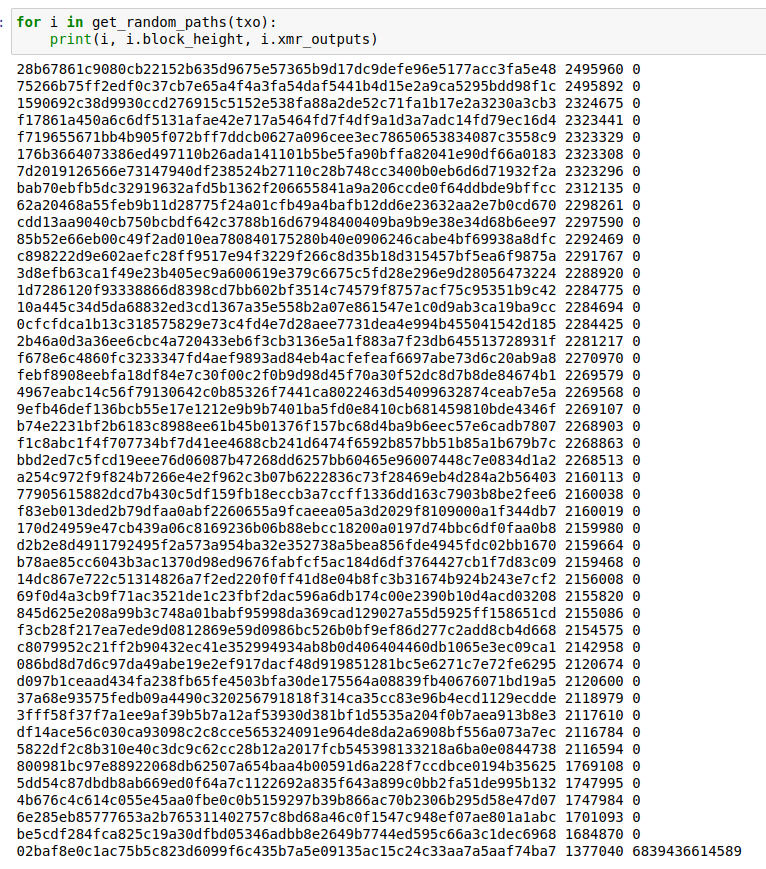
\includegraphics[scale=0.5]{randompath}

An additional statistical choice is that of Bayesian Networks, where distributions are defined over the various structures: like the edges, vertices, and faces.  For example, although a transaction is of unknown value on the Monero blockchain, this very transaction value could be the subject of a leaked transaction.  Even without the leak the transaction value is constrained by the number of coinbase transactions that eventually lead to its inputs, as decoys or otherwise.  The Bayesian framework is a natural choice to incorporate the information gain from this conditioned information.  We will elaborate in the computational framework section where we introduce the computational tools to actually perform these tasks \cite{patil2010pymc}.

\textcolor{red}{
Although I haven't completely converged on selecting the exact perspective, progress has been made on both the Bayesian and TDA theoretical fronts.  I have been able to do without the `bipartite' nature of the graphs, insisting on vertices of all the same varietal, namely just the transactions.  
}

\textcolor{red}{The main idea of TDA is the notion of `persistence.'  A parameter is sweeped and the topological features are tracked as that filtration takes place.  In this setting there are a number of ways to consider this filtration.  First off, a parameter can be sweeped from top to bottom or from bottom to top.  The two natural choices for filtration are by probability or by time (block height), and seems to make the most sense sweeping from high probability to low probability or from current time back towards the genesis block.  These two filtrations are largely the same here since it happens to be the case that Monero chooses from recent blocks moreso than old blocks for the decoy selection.
}

\textcolor{red}{
I've been exploring the effect of treating the RingCT as a simplicial complex of transactions.  Consider a typical ring of a typical transaction:
}

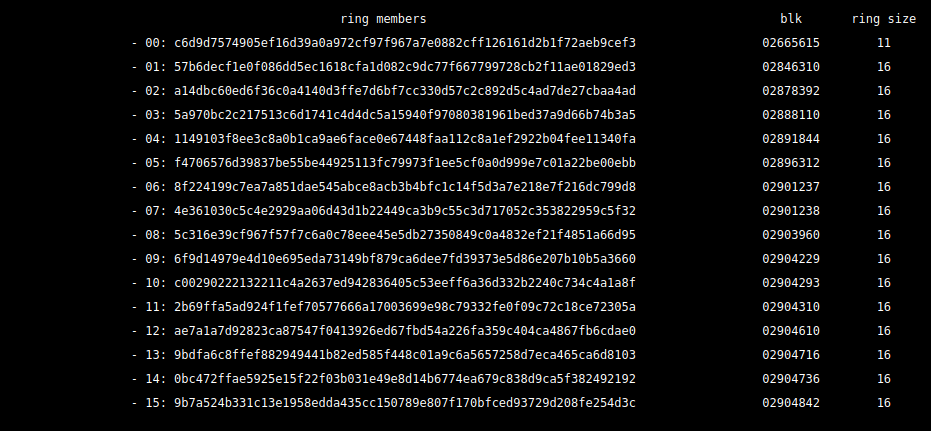
\includegraphics[scale=0.5]{ringct}

\textcolor{red}{The full simplicial complex for this ring includes the 16 vertices, $tx_{15}$, ..., $tx_0$, the edges $(tx_{15}, tx_{14})$, ..., $(tx_1, tx_0)$, the planes $(tx_{15}, tx_{14}, tx_{13})$,...,$(tx_2,tx_1,tx_0)$, the tetrahedron $(tx_{15}, tx_{14}, tx_{13}, tx_{12})$, ... and so on until you have the 16 dimensional simplex $(tx_{15}, tx_{14}, tx_{13}, ..., tx_0)$.  The simplex value to assign is the youngest block height in the simplex, for e.g. $(tx_{15}, tx_{14}, tx_{13}, tx_{12})$, would have the value 2904610.}

\textcolor{red}{There might be little motivation to keep all 16 dimensional simplices; the main advantage is it would allow for the presence of non-trivial persistent homology of up to order 15 while the main disadvantage is the additional bookkeeping.  The two most important being the zeroth order, which identifies the connected components, and the first order which identifies the circuits.  Strictly speaking we only need up to two orders of persistent homology to detect the birth and death of the components and cycles needed for the EAE attacks, but the higher order homologies might be informative in unknown ways.}
 
\textcolor{red}{I am also using TDA in the construction and the analysis of the Taint Tree.  For a given transaction, the collection of all possible histories can be enumerated, or at least sampled.  I am interested into how the likelihoods of the paths cluster.  Plotting all these likelihoods on a number line forms a spectrum of sorts; do these probabilities cluster at all into highly likely, possible, or rare?  Ideally the decoy selection process would make this spectrum fairly flat, but my initial investigation suggests there is some structure to it.}

\textcolor{red}{The large scale remaining to do here is to calculate the intersections of these taint trees via topological methods}
  
\section{Computational Framework}

The power of TDA comes through its use of Persistent Homology.  A filtration is introduced to enable the calculation of a persistence diagram which quantifies noise and structures at all hierarchical levels.  In the setting of Monero the scalar parameter behind this filtration can be the 'probability of being the real transaction.'   As this probability parameter is sweeped from zero to one various topological features come and go.  The interval of the parameter where these features 'persist' is the subject of persistent homology.  These persistence diagrams reside in a metric space where the distance is given by the Wasserstein distance. It will be the object of the proposed research to formalize these ideas but we would like to sketch our initial approach.

Although the graph of the entire Monero blockchain is large, it may be within the realm of computational feasibility that a graph analysis is performed on the entire blockchain.  Furthermore the subgraphs that arise out of the aided information in the case of the overseer attacks would be tractable computationally and we can presume readily available to an adversary, thus it is necessary to understand what information could have been leaked.  

To move some of the theoretical work into the realm of a messy reality various packages are available, some of which will also be useful and appropriate in the Empirical Framework section.   In my previous explorations of the subject I felt as though having rings composed of entirely decoys (removing the ability to know for certain that some input was being spent) or having decoy outputs (red-herring outputs where the entire subsequent taint tree is obfuscating the truth) would be very problematic for blockchain analysts.  With two outputs, both parties are of microeconomic interest; both were involved in the transaction.  Adding additional decoy outputs not only provides more choices in subsequent transactions, but insures that these choices are working towards the obfuscation of the transaction graph.  These and other hypothesis can be explored. 

\textcolor{red}{A python library has been started to interface with the blockchain, construct the various simplices, and compute the various homologies.  The main dependencies are \textit{pymc, pot (python optimal transport)}.  The TDA has been performed in pure python at the moment, trying to identify the circuits using intersections, will be migrating to some tda package (probably giotto-tda).}
  

\section{Empirical Framework}

In a previous study \cite{Borggren2020}, \cite{Borggren2020a} we staged a Monero blockchain with 10-50 agents interacting with each other to probe connectivity of the resulting transactions.  The machine learning therein was followed up on in another Magic Grant funded project \cite{jack}.  I think the similar research going forward should utilize the test network rather than building a new blockchain from scratch.  I would also like to draw attention to the correlation results therein, it signifies a new attack not addressed by the decoy system in use.  

The Monero test network and stage net will be used to perform an empirical analysis of example Overseer attacks to avoid transaction costs and other considerations.  Cat-and-Mouse games will be setup to mimic various microeconomic considerations in analogy to the attacks:

\begin{itemize}
	\item Sender repeats transactions to a Receiver on a schedule.
	\item Receiver aggregates a collection of previous transactions on a timed schedule 
	\item Receiver aggregates a collection of previous transactions when a threshold amount has been reached.
	\item Sender sends transactions to a collection of addresses in hopes to identify which addresses belong to a particular user.
\end{itemize}

the resulting transaction graphs can then be analyzed and algorithm performance evaluated.  It is possible that the decoy selection process may require such graph analysis, drawing from specific clusters in order to increase the fungibility between the clusters.  We aim to connect and contribute to other ongoing Monero Research Lab research as fitting and able.

If the effort can be done safely, so as not to compromise existing consumers, the real Monero blockchain can also be analyzed.  Motifs can be identified and histogrammed and previous leaks and residue from previous forks can be analyzed to see to what extent the blockchain has already been compromised.  Churning strategies can be recommended or decoy selection can be motivated to diffuse this information loss over the continuing blockchain.

\textcolor{red}{Bayesian stats were used in a variety of ways, starting with the fitting of the decoy distributions.  A number of updates have been made to Monero since the last time I worked on it.  The RingCT has gone from 11 to 16 and the decoy algorithm has improved.  To evaluate the various probabilities of paths a clear understanding of how the decoy selection is made is required.  I am still after this clear understanding, but this is the picture I've put together so far.  Using the python package pymc (formerly pymc3) a (log of) `Beta' distribution was fit to historic data.  A couple of observations were made understanding the decoy selection.  First note that the support for the Beta function is 0 to 1, so there is some subtlety into how the decoys are selected, the 0 corresponds to the genesis block and the 1 corresponds to the current block.  I'm pretty sure the net effect of the `log' beta remark in the codebase is that a draw from the beta distribution returns a number between 0 and 1, multiplying that by the current block height and rounding to an integer gives the decoy block height.  The time stretching reminds one of the expansion of the universe. An adjustment that has been made in recent years is that the actual decoy selection used isn't a simply beta function, but there seems to be a window of recent transactions, where the beta distribution switches to a flat distribution.  From my initial analysis it seems that this is doing well at the desired effect of mixing among the recent transactions.}
\textcolor{red}{The results from the empirical fits gave values consistently above the $19.38$, $1./61$ factors suggested in the codebase.  Typical fits over 2000 blocks are shown here.  We will use these empirical fits to evaluate our probabilities for the time being, but have as a lower priority to-do to also fit the additional parameter of when the distribution turns flat.  This cursory examination suggests choosing very old transactions is exceedingly rare.}

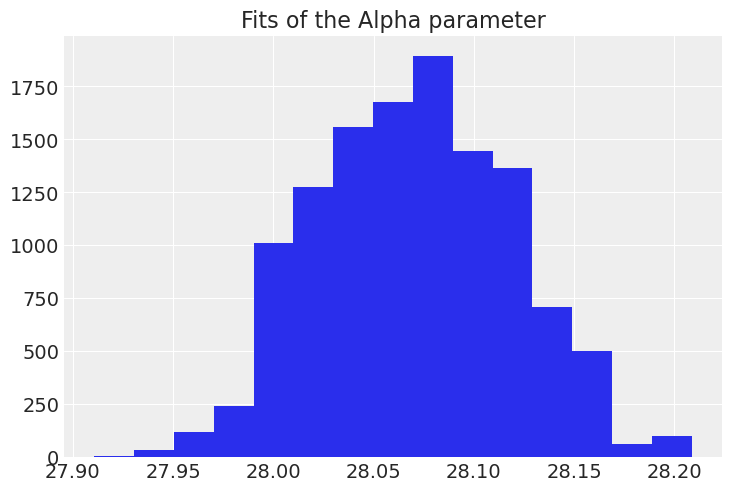
\includegraphics[scale=0.5]{alpha}

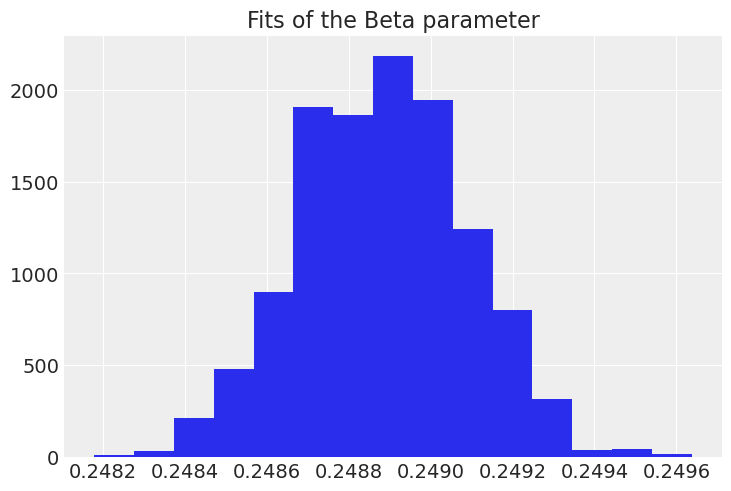
\includegraphics[scale=0.5]{beta}

\textcolor{red}{We also show what the measured values look like, and what the distributions expected from the fit and expected distributions look like.}

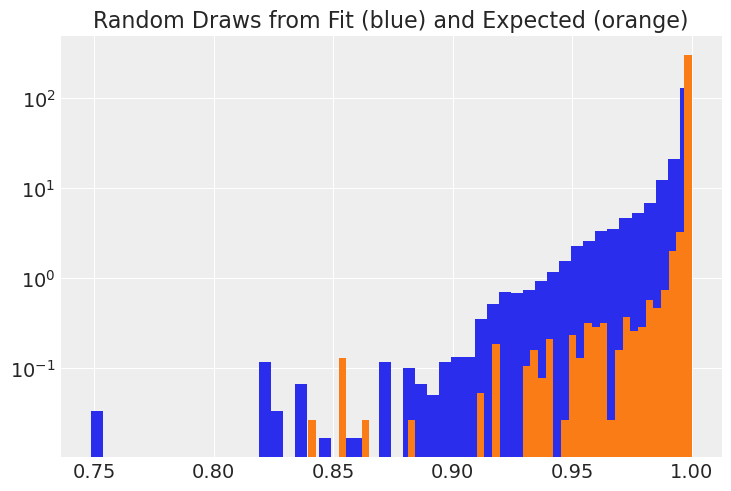
\includegraphics[scale=0.5]{fit}

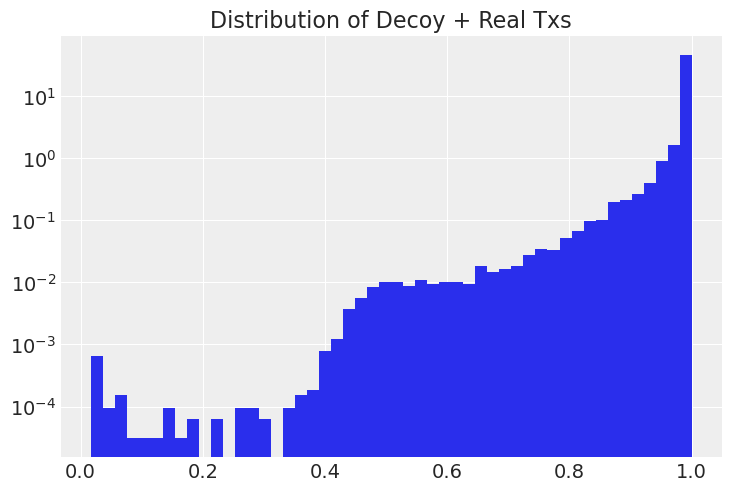
\includegraphics[scale=0.5]{decoyreal}



\section{Integrating the Frameworks}

Although it is the subject of the research to fully formalize these ideas, we can begin to see how the research may unfold and how the insights from the different approaches integrated.  The information garnished from these analysis are of different varietals, deterministic, Bayesian, frequentist.  Some aspects of which are more important depending on the questions being asked and the motives of those asking them.  For example some level of de-anonymization might be sufficient to get a picture of what the microeconomic activity occurring on the blockchain is like but insufficient to identify or link the specific entities involved.

The graph theoretical and TDA approaches, in their basic form, are deterministic theories, they can potentially reveal certainties with respect to connectivity.  The Monero blockchain itself, after many statistical choices like decoy selection, stealth address creation are made become part of Natural History, a fossil record of the specific things that occurred.  It is a basic premise of Monero that `the one true subgraph' consisting of all real transactions between real users can be sufficiently obfuscated with decoys, hidden in plain sight, so as to be rendered indiscoverable.  The performance of this hypothesis in real world conditions versus powerful mathematical and computational machinery is what we are seeking to address.  These conditions involve zooming into a potentially very small subset of transactions and diligently using all available resources to prune this tree into a clear picture of economic activity.  

Indeed the fear behind the Overseer Attack is that these 'red-handed' connections can be made given enough leaked information.  In the same way a user has certainty over the transactions involved in their own activity, can an exchange achieve that same level of certainty on the origins of some funds through the systematic pruning of the edges their privileged information enables?  This question can be asked deterministically and addressed through theoretical and empirical means.  In which case the graph/simplex decompositions results in either a unique explanation of the scenario or a subgraph which still has a host of decoys present.  This latter case is the more general case and the one anticipated by myself and others.  

As mentioned in \cite{MiersZcash} this level of certainty isn't obligatory for the purveyors of these attacks and they may proceed with their queries at the level of probability of their choosing.  At this stage we introduce probabilities and ask how the weights have changed on the decoy sets with the conditioned information.  In the setting of Overseer Attack this investigation may take on similarities of the motif-hunting in \cite{ranshous2017exchange} with the added calculation of likelihoods that these motifs and their subgraphs originated from the decoy selection process.  A narrative of accuracy also begins when these probabilities get introduced.  A bias towards recall over precision can be present in the case where False positives are of little importance; if the unscrupulous-attack-purveyor is not as much concerned with busting down the wrong door so much as the time wasted in the process.  It is thus important to evaluate algorithms over the spectrum of relative priority between false positives and false negatives; algorithms with a high rate of false positive can still be quite dangerous for victims of these attacks.

It is most natural to think of how that evaluation process would proceed in the empirical framework section.  We will actually try to execute a statistically significant number of these attacks on our own test network.  Having the blockchain data as well as the private wallet data will allow us to evaluate the performance of yet-to-be-determined algorithms and mathematics and considering the false positive and false negative rates.  Simulating the scenarios as well will allow us to establish a ground truth off of which our recommendations can be tested and evaluated.  

\section{Proposal Request}

The author is seeking a rate of 2/3 of 1 XMR/hour or approximately $\$100/hour$ and has the means to put up to a full time effort (30-40 hours/week) in June-July 2023 and a part time effort thereafter of approximately 15-20 hours/week.  This rate is slightly less than the author's usual rate for data science work at the PhD level, but commensurate with previous funding from the Magic Fund.  The rate is also less than comparable work at Chainalysis, Elementus, TRM Labs, and US Government whose ongoing work on Monero analysis does not necessarily feedback into the improvement of the protocol and indeed can be antithetical to the currency's objective.  The total request is \textbf{220 XMR} over three months.  Although this total is larger than a typical reward perhaps it can be combined with CCS or other mechanisms and is a competitive bid for the requested work.

This timeline is short compared to usual peer-reviewed research timescales but I think is sufficient amount of time to understand the breadth and depth of the issues and inform the Monero community of a path forward.  It should also be clear at the end of this time if the Monero Foundation is interested into continuing the research, at which time new proposals can be submitted and further funding arrangements made as it sees fit.

I'd like to acknowledge the anonymous Monero community members that reached out to others and myself in order to create a small community of Monero/Graph Theory/Statisticians who have expressed interest and capabilities towards the problems these adversarial attacks present.  Although this proposal does not seek particulars of the funding arrangements for those researchers, I will be grateful and open to their continuous feedback throughout the research process and contributing feedback to their efforts.  My research efforts for the entire duration of the proposed work will be transparent to this working group to facilitate this feedback loop.  

Part of the partitioning into \textit{Theoretical, Statistical, and Empirical} components is to be able to scale the effort in a multitude of directions based on the needs of the community as well as the interests and capabilities of the other interested researchers.  Having lead teams of data scientists from prestigious universities with skill levels from undergraduate, graduate, post-doc and even professorial levels, I feel equipped and available to lead the effort of scaling these analysis to whatever level the community deems appropriate.  

\section{Update}
Versions of this proposal were released to the working group mentioned as well as the Monero Research Lab matrix channel.  Isthmus, Xmrack and Rucknium responded with feedback.  There seems to be a preference for using the transaction graph of the real network as opposed to the test network.  My worry of compromising other transactions through the analysis of our own seemed not to be shared.  Doing the tests on the real network would be fine but would take cooperation and some Monero to provide those transactions.  I don't personally want to steward Monero beyond dust transactions for this purpose, but perhaps the foundation or users who are willing to share transaction history from their wallets can help play the role of E, A, as well as B in the EABE attacks.  It is my belief at this stage that the patterns created by these attacks will be consistent on either the test network or the real network, but that the patterns may be more `hidden' with the added transactions on the real network.  

My assertion about the timeline being short was also seconded, and third-ed.  Analogous government contracts would likely be for a year, and indeed 6 months to 1 year might be more reasonable for true resolution of these issues.  I am just trying to be consistent with the previous award amounts, but would be delighted to continue the work for longer at the same rate.  I would certainly agree to \textbf{440 XMR} over 6 months as well, but wanted to give the foundation the option to make an assessment early in the research, and also an opportunity for the researchers that are enthusiastic about helping me with this work to apply and be compensated for their efforts as well. 

\textcolor{red}{Continuing I will be trying to formalize and measure the various EAE attacks which I will organzize and enumerate.  So far I have been trying to detect candidate EAE patterns in the blockchain, given labels I will try to mimic an exchange trying to identify their particular customer out of a host of possible patterns.}
  
\bibliography{monero}
\bibliographystyle{unsrtnat}

\end{document}

